\begin{refsection}

\chapter{U--Th--He and fission tracks}\label{ch:thermochron}

The U--Th--He and fission track methods are two relatively new
chronometers that were never implemented in \citet{ludwig2003}'s
~\texttt{Isoplot} program.  Despite their short history, the
statistical treatment of the U--Th--He method and especially the
fission track method are well developed and in some ways more advanced
than that of more established geochronometers. For example, both the
radial plot of Section~\ref{sec:radial} and the mixture models of
Section~\ref{sec:mixtures} were originally developed for fission track
data \citep{galbraith1990a,galbraith1990b}, but are generalised to all
chronometric methods by \texttt{IsoplotR}. And in this chapter we will
see that the U--Th--He method was the first to be cast in a logratio
context \citep{vermeesch2010a}, which is slowly being adopted by other
chronometers and promises to become even more important in the future.

\section{U--Th--(Sm)--He}\label{sec:advancedUThHe}

\texttt{IsoplotR} offers a single input format for U--Th--(Sm)--He
data, which constitutes a simple table with the following columns:

\begin{center}
He, err[He], U, err[U], Th, err[Th], Sm, err[Sm]
\end{center}

\noindent which contains all the necessary information to calculate
the age. Rewriting Equation~\ref{eq:U-Th-He}:
\begin{equation}
\begin{split}
  \left[^4\mbox{He}\right] = & ~a(t) 
   \mbox{[U]} + b(t)\mbox{[Th]} + c(t)\mbox{[Sm]} \\
   \mbox{where~} a(t) = &
   \left[8 \frac{137.818}{138.818} (e^{\lambda_{238}t} - 1) +
     7 \frac{1}{138.818} (e^{\lambda_{235}t} - 1) \right] \\
   b(t) = & ~6 (e^{\lambda_{232}t} - 1)\\
    \mbox{and~} c(t) = & ~0.1499 (e^{\lambda_{147}t} - 1)
\end{split}
\label{eq:UThHe2}
\end{equation}

Because Sm (1) produces only one \textalpha-particle per decay event;
(2) has a very long half-life; and (3) its radioactive isotope 147
only accounts for 14.99\% of total samarium, Sm can be ignored as a
parent in all but the most Sm-rich samples. For this reason, some
laboratories do not measure Sm at all, and the `Sm' and `err[Sm]'
columns are optional. If omitted, \texttt{IsoplotR} will simply assume
that the Sm-concentration is zero.\\

The He, U, Th (and Sm) measurements must be expressed in internally
consistent \textbf{atomic units} such as mol, fmol, pmol, mol/cc,
fmol/\textmu{g} etc. They must not be expressed in mass units such as ppm,
ppb or wt\%! For U and Sm, which are poly-isotopic elements, it is the
total amount that is required, and not just \textsuperscript{238}U and
\textsuperscript{147}Sm. A second important requirement is that the
data have been corrected for $\mathbf{\alpha}$\textbf{-ejection} prior
to analysis, as explained in the next section.

\section{The \textalpha-ejection correction}

Like argon, helium is a noble gas that is lost to the environment (and
eventually to space) at high temperatures by volume diffusion.
Additional complication is added by the physical separation of the
parent and daughter nuclides in the U-Th-(Sm)-He system. This
separation results from the energy released during \textalpha-decay,
which displaces the \textalpha-particles by up to 16~\textmu{m} and may
result in the ejection of helium produced by parent atoms that are
sited near the edges of the host mineral. That lost helium must be
taken into account when interpreting the thermal history of a
sample. For rapidly cooled samples, this can be done by applying a
geometric correction to the U, Th and Sm-measurements. For a sphere:
\begin{equation}
  F_T = 1 - \frac{3}{4}\frac{S}{R} + \frac{1}{16} \left[\frac{S}{R}\right]^3
    \label{eq:FTsphere}
\end{equation}

\noindent where $F_T$ is the fraction of helium that is retained in
the grain, $r$ is the radius of a sphere with equivalent
surface-to-volume ratio as the mineral habit of interest, and $S$ is
the \textalpha-stopping distance:

\begin{center}
\begin{tabular}{cccccc}
  mineral & \textsuperscript{238}U & \textsuperscript{235}U
  & \textsuperscript{232}Th & \textsuperscript{147}Sm \\ \hline
  apatite & 18.81 & 21.80 & 22.25 & 5.93 \\
  zircon & 15.55 & 18.05 & 18.43 & 4.76 \\
  sphene & 17.46 & 20.25 & 20.68 & 5.47
\end{tabular}
\captionof{table}{\textalpha-stopping distances ($S$) in \textmu{m}.}
\label{tab:stoppingdistances}
\end{center}

Most minerals are not spherical but elongated prismatic, and can be
approximated to a first degree as cylinders with radius $r$ and height
$h$:
\begin{equation}
  F_T = 1 - \frac{1}{2}\frac{(r+h)S}{rh} +
  0.2122 \frac{S^2}{rh} + 0.0153 \frac{S^3}{r^3}
  \label{eq:FTcylinder}
\end{equation}

An extensive list of formulas for even more realistic geometric shapes
is provided by \citet{ketcham2011}. The \textalpha-ejection correction
can be applied in one of three ways:

\begin{enumerate}
\item For relatively young ($<100$~Ma) samples, the ejected helium can
  be mathematically replaced to a good approximation by dividing the
  uncorrected U--Th--He age by $F_T$ \citet{farley2002}:
  \begin{equation}
    t^* \approx \frac{t}{
      \frac{a(t^*)[U]}{a(t^*)[U]+b(t^*)[Th]}
      \left(
      \frac{137.818}{138.818} F_T^{238} +
      \frac{1}{138.818} F_T^{235}
      \right) + 
      \frac{b(t^*)[Th]}{a(t^*)[U]+b(t^*)[Th]} F_T^{232}
    }
    \label{eq:alphacorr1}
  \end{equation}

  \noindent where $t^*$ is the corrected age; $a(t^*)$ and $b(t^*)$ are
  defined in Equation~\ref{eq:UThHe2}; and $F_T^{238}$, $F_T^{235}$
  and $F_T^{232}$ are the \textalpha-retention factors of
  \textsuperscript{238}U, \textsuperscript{235}U and
  \textsuperscript{232}Th, respectively.
\item More accurate results are obtained by dividing not the age but
  the helium concentrations by the \textalpha-retention factor
  \citep{min2003, vermeesch2008a}:
  \begin{equation}
    [\mbox{He}^*] = \frac{[\mbox{He}]}{
      \frac{a(t^*)[\mbox{U}]}{a(t^*)[\mbox{U}]+b(t^*)[\mbox{Th}]}
      \left(
      \frac{137.818}{138.818} F_T^{238} +
      \frac{1}{138.818} F_T^{235}
      \right) + 
      \frac{b(t^*)[\mbox{Th}]}{a(t^*)[\mbox{U}]+b(t^*)[\mbox{Th}]} F_T^{232}
    }
    \label{eq:alphacorr2}
  \end{equation}
  \noindent and then plugging [He$^*$] into Equation~\ref{eq:UThHe2}
  instead of [He]. The difference between
  Equations~\ref{eq:alphacorr1} and \ref{eq:alphacorr2} can reach
  several percent for early Precambrian ages.
\item The most accurate approach to \textalpha-ejection correction is to
  adjust not the radiogenic daughter product but the radioactive
  parents:
  \begin{equation}
      [{}^{238}\mbox{U}^*] = \frac{[{}^{238}\mbox{U}]}{F_T^{238}},~
      [{}^{235}\mbox{U}^*] = \frac{[{}^{235}\mbox{U}]}{F_T^{235}},~
      \mbox{~and~} [{}^{232}\mbox{Th}^*] =
      \frac{[{}^{232}\mbox{Th}]}{F_T^{232}}
    \label{eq:alphacorr3}
  \end{equation}
  \noindent and then substituting [\textsuperscript{238}U$^*$],
            [\textsuperscript{235}U$^*$] and [\textsuperscript{232}Th$^*$]
            for [\textsuperscript{238}U], [\textsuperscript{235}U] and
            [\textsuperscript{232}Th] in Equation~\ref{eq:UThHe2}.
\end{enumerate}

\texttt{IsoplotR} assumes that the \textalpha-ejection correction has
been applied to the data \textbf{prior} to age calculation. This must
be done using either method 2 or 3 above.

\section{isochrons}

More often than not, and more often than for other geochronometers,
U-Th-(Sm)-He data are overdispersed with respect to the analytical
uncertainties. Several mechanisms have been invoked to explain this
overdispersion, including compositional effects, radiation damage, and
breakage during mineral separation.\\

\texttt{IsoplotR} implements four different ways to visualise, average
and quantify the overdispersion.  The first two of these are the
weighted mean and radial plot, which were discussed in
Sections~\ref{sec:weightedmean} and \ref{sec:radial}. The third way is
the isochron plot and age. This uses a first order approximation of
the U--Th--He age equation:
\begin{equation}
  t \approx \frac{\left[{}^{4}\mbox{He}\right]}{P} \mbox{,~where~} P =
  \left[8 \frac{137.818}{138.818} \lambda_{38} + 7 \frac{1}{138.818}
    \lambda_{35} \right] [\mbox{U}] + 6 \lambda_{32} [\mbox{Th}]
    \label{eq:t=HeP}
\end{equation}

\noindent which is accurate to better than 1\% for ages less than
100~Ma \citep{vermeesch2008a}. A U--Th--He isochron is constructed by
plotting the numerator of the right-hand side of
Equation~\ref{eq:t=HeP} against the denominator and fitting a straight
line through several aliquots of the same sample:\\

\noindent\begin{minipage}[t]{.4\linewidth}
\strut\vspace*{-\baselineskip}\newline
\includegraphics[width=\textwidth]{../figures/UThHeisochron.pdf}\\
\end{minipage}
\begin{minipage}[t]{.6\linewidth}
  \captionof{figure}{U--Th--He isochron with a model-3 fit. Because
    the parent and daughter nuclides are analysed separately on
    different mass spectrometers, their uncertainties are uncorrelated
    with each other. Hence the data are shown as error crosses instead
    of error ellipses.}
  \label{fig:UThHeisochron}
\end{minipage}

\section{Compositional data analysis and the `helioplot'}

The fourth and final way to visualise and average U--Th--He data is
based on the fact that U, Th and He are \emph{compositional}
data. This means that it is not so much the absolute concentrations of
these elements that bear the chronological information, but rather
their relative proportions. Equation~\ref{eq:UThHe2} can be recast in
terms of the elemental ratios U/He, Th/He, which take on strictly
positive values:
\begin{equation}
  a(t) \frac{[\mbox{U}]}{[\mbox{He}]} +
  b(t) \frac{[\mbox{Th}]}{[\mbox{He}]} = 1
\end{equation}

The space of all possible U--Th--He compositions fits within the
constraints of a ternary diagram. If Sm is included as well, then this
expands to a three-dimensional tetrahedral space
\citep{vermeesch2008a}. The \textbf{central age} is obtained by first
computing the average U--Th--He composition of a multi-sample dataset,
and then calculating the U--Th--He corresponding to that composition.
This is a similar procedure in a sense to the two-step process that
was used to compute concordia ages in Section~\ref{sec:concordia}.
Unfortunately, averaging compositional data is not as straightforward
as one may think. Consider, for example, the following ternary
dataset:\\

\noindent\begin{minipage}[t]{.4\linewidth}
\strut\vspace*{-\baselineskip}\newline
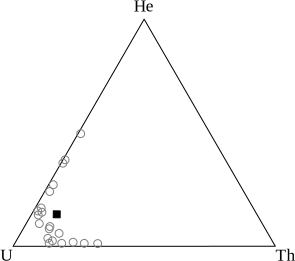
\includegraphics[width=\textwidth]{../figures/ternaryhelium.pdf}\\
\end{minipage}
\begin{minipage}[t]{.6\linewidth}
  \captionof{figure}{The U--Th--He age equation is scale invariant in
    the sense that the three elements can be renormalised to unity
    without loss of chronological information. This figure shows a
    synthetic dataset of 20 scattered U--Th--He measurements (grey
    circles). The arithmetic mean composition of the dataset is shown
    as a black square. It plots outside the data cloud, and is
    therefore not representative of the data.\\}
  \label{fig:ternaryhelium}
\end{minipage}

\citet{aitchison1986} showed that the natural way to process
compositional data is by subjecting them to a \textbf{logratio
  transformation}. In the case of the U--Th--He system, the logratio
analysis is achieved by first defining two new variables:
\begin{equation}
  u \equiv \ln\!\left(\frac{\mbox{[U]}}{\mbox{[He]}}\right),
  v \equiv \ln\!\left(\frac{\mbox{[Th]}}{\mbox{[He]}}\right)
  \label{eq:alr}
\end{equation}

\noindent and then performing the desired statistical analysis
(averaging, uncertainty propagation, ...) on the transformed
data. Upon completion of the mathematical operations, the results can
then be mapped back to U-Th-(Sm)-He space using an inverse logratio
transformation:
\begin{equation}
    [He] = \frac{1}{\left[e^{u}+e^{v}+1\right]},~
    [U] = \frac{e^{u}}{\left[e^{u}+e^{v}+1\right]},~
    [Th] = \frac{e^{v}}{\left[e^{u}+e^{v}+1\right]}
    \label{eq:ialr}
\end{equation}

\noindent where [He] + [U] + [Th] = 1.\\

\noindent\includegraphics[width=\linewidth]{../figures/alr.pdf}
\begingroup
\captionof{figure}{The logratio transformation maps data from an
  $n$-dimensional compositional space to an $(n-1)$-dimensional
  Euclidean space. For the U--Th--He data, it maps the data from a
  ternary diagram ($n=3$) to a bivariate ($n-1=2$) dataspace using
  Equation~\ref{eq:alr}. In this transformed space, it is safe to
  calculate the arithmetic mean (black square) and confidence regions
  (black ellipse). After completion of these calculations, the result
  can be mapped back to the ternary diagram using the inverse logratio
  transformation (Equation~\ref{eq:ialr}).\\}
\label{fig:alr}
\endgroup

In the context of U--Th--He dating, the central age is defined as the
age that corresponds to the arithmetic mean composition in logratio
space. \texttt{IsoplotR}'s \texttt{helioplot} function performs this
calculation using the same algorithm that is used to obtain the
weighted mean U-Pb composition for the concordia age calculation
(Section~\ref{sec:concordia}).\\

\noindent\begin{minipage}[t]{.7\linewidth}
\strut\vspace*{-\baselineskip}\newline
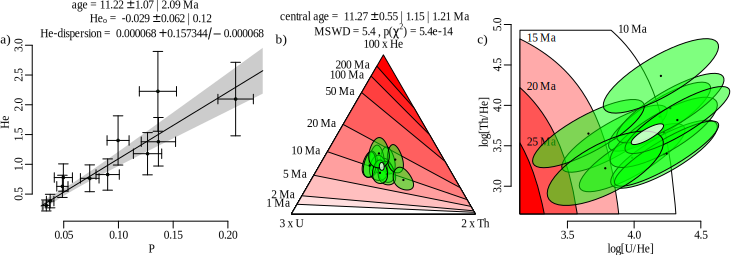
\includegraphics[width=\textwidth]{../figures/helioplot.pdf}\\
\end{minipage}
\begin{minipage}[t]{.3\linewidth}
  \captionof{figure}{a) ternary diagram and b) logratio diagram or
    `helioplot' of the U--Th--He data from
    Figure~\ref{fig:UThHeisochron}. The white ellipse marks the
    (geometric) mean U--Th--He composition.\\}
  \label{fig:UThHeIsochronHelioplot}
\end{minipage}

Overdispersion is treated similarly as in a regression context
(Section~\ref{sec:regression}).  Thus, there are options to augment
the uncertainties with a factor $\sqrt{\mbox{MSWD}}$ (model-1); to
ignore the analytical uncertainties altogether (model-2); or to add a
constant overdispersion term to the analytical uncertainties
(model-3).  The helioplot diagram provides a convenient way to
simultaneously display the isotopic composition of samples and their
chronological meaning. In this respect, they fulfil the same purpose
as the U--Pb concordia diagram (Section~\ref{sec:concordia}) and the
U--series evolution plot (Section~\ref{sec:ThUevolution}).

\section{Fission tracks}\label{sec:fissiontracks}

\texttt{IsoplotR} accepts three types of fission track data:

\begin{enumerate}
\item{`EDM':} \textzeta, err[\textzeta],
  \textrho\textsubscript{D}, err[\textrho\textsubscript{D}], 
  N\textsubscript{s}, N\textsubscript{i}
\item{`ICP (\textzeta)':} \textzeta, err[\textzeta], spot size
  (\textmu{m}), U\textsubscript{1}, err[U\textsubscript{1}],
  U\textsubscript{2}, err[U\textsubscript{2}], $\ldots$,
  U\textsubscript{n}, err[U\textsubscript{n}]
\item{`ICP (absolute)':} spot size (\textmu{m}), U\textsubscript{1},
  err[U\textsubscript{1}], U\textsubscript{2},
  err[U\textsubscript{2}], $\ldots$, U\textsubscript{n},
  err[U\textsubscript{n}]
\end{enumerate}

\noindent \textzeta, err[\textzeta], \textrho\textsubscript{D},
err[\textrho\textsubscript{D}], and spot size are scalars, and
N\textsubscript{s}, N\textsubscript{i} and U\textsubscript{i} and
err[U\textsubscript{i}] are vectors. The three formats represent two
different approaches to fission track dating:

\begin{enumerate}
\item The External Detector Method (EDM) implements the neutron
  irradiation method that was previously introduced in
  Section~\ref{sec:fission-tracks}.
\item The `ICP' method uses LA-ICP-MS (see
  Section~\ref{sec:mass-specs}) to determine the
  \textsuperscript{238}U-content of fission track samples.  The main
  reasons for this change are the increased throughput achieved by not
  having to irradiate samples and the ease of double-dating apatite
  and zircon with the U-Pb method.
\end{enumerate}

\section{The external detector method}
\label{sec:EDM}

Recall the fission track age equation from
Section~\ref{sec:fission-tracks}:
\begin{equation}
t =
\frac{1}{\lambda_{38}}\ln\left(1+\frac{g_i}{g_s}
\lambda_{38}\zeta\rho_d\frac{N_s}{N_i}\right)
\label{eq:tzeta2}
\end{equation}

As mentioned at the beginning of this chapter, the fission track
method has been a test bed of statistical approaches that have
subsequently been adopted by other chronometers. A case in point is
the radial plot, which is uniquely suited to deal with the large and
highly variable (`heteroscedastic') counting uncertainties of fission
track data. Spontaneous fission is accurately described by a Poisson
distribution. For young and/or uranium-poor samples, there is a finite
probability that the spontaneous track count is zero for some grains.
To accommodate such zero values, it is customary to use an arcsin
transformation for radial plots instead of the usual logarithmic
transformation \citep{galbraith1990a}:
\begin{equation}
z_j = \arcsin\sqrt{\frac{N_{sj} + 3/8}{N_{sj}+N_{ij}+3/4}}
\label{eq:zj}
\end{equation}

\noindent and
\begin{equation}
\sigma_j = \frac{1}{2\sqrt{N_{sj}+N_{ij}+1/2}}
\label{eq:sj}
\end{equation}

The arithmetic mean is not a reliable estimator of the true age, for a
similar reason why the arithmetic mean is not the best estimator of
the average U--Th--He composition and age. The Poisson distribution is
negatively skewed, and this biases the arithmetic mean. The solution
is similar as for the U--Th--He, namely:

\begin{enumerate}
\item Take the average logarithm of the spontaneous and induced
  track densities.
\item Compute the fission track age the corresponds to this average
  ratio.
\end{enumerate}

This procedure again gives rise to a `central age'. Fission track data
are often overdispersed with respect to the Poisson counting
uncertainties, and this dispersion carries important thermal history
information. It is therefore customary to compute the average track
density ratio using a model-3 style random effects model, in which the
true $\rho_s/\rho_i$-ratio is assumed to follow a log-normal
distribution with location parameter $\mu$ and scale parameter
$\sigma$ \citep{galbraith1993}:
\begin{equation}
\ln\left[\frac{\rho_s}{\rho_i}\right] \sim \mathcal{N}(\mu,\sigma^2)
\label{eq:logrhosrhoi}
\end{equation}

This model gives rise to a two-parameter log-likelihood function:
\begin{equation}
  \mathcal{L}(\mu,\sigma^2) = \sum\limits_{j=1}^{n}
  \ln f_j(\mu,\sigma^2)
\label{eq:Lcentral}
\end{equation}

\noindent where the probability mass function $f_j(\mu,\sigma^2)$ is
defined as:
\begin{equation}
  f_j(\mu,\sigma^2) = {{N_{sj}+N_{ij}}\choose{N_{sj}}}
  \int\limits_{-\infty}^{\infty} \frac{e^{\beta N_{sj}} \left( 1 +
    e^\beta \right)^{-N_{sj}-N_{ij}}} {\sigma\sqrt{2\pi}
    e^{(\beta-\mu)^2/(2\sigma^2)}} d\beta
  \label{eq:fjms}
\end{equation}

\noindent in which the fission track count ratios are subject to two
sources of variation: the Poisson counting uncertainty and an
`(over)dispersion' factor $\sigma$.  Maximising Eq. \ref{eq:Lcentral}
results in two estimates $\hat{\mu}$ and $\hat{\sigma}$ and their
respective standard errors.  Substituting $\exp[\hat{\mu}]$ for
$N_s/N_i$ in Equation~\ref{eq:tzeta2} produces the desired central
age. $\hat{\sigma}$ estimates the overdispersion, and quantifies the
excess scatter of the single grain ages which cannot be explained by
the Poisson counting statistics alone. This dispersion can be just as
informative as the central age itself, as it encodes geologically
meaningful information about the compositional heterogeneity and
cooling history of the sample.  In the absence of excess dispersion,
i.e. if $\hat{\sigma}$=0, the central age equals the pooled age, so
there is not really any reason to use the pooled age at all.

\section{LA-ICP-MS based fission track dating}
\label{sec:ICPFT}



\section{Compositional zoning and zero track grains}
\label{sec:zerotracks}

Equation~\ref{eq:tzeta2} represents a classic case of a `matched
pairs' experimental design \citep{galbraith2010}. By counting the
spontaneous and induced tracks over exactly the same area, the age
calculation reduces to a simple comparison of two Poisson-distributed
variables ($N_s$ and $N_i$). This enables an explicit maximum
likelihood formulation, which greatly simplifies all subsequent
statistical analyses. As a result, it is fair to say that the fission
track method represents the gold standard among geochronometers in
terms of statistical rigour.\\

Abandoning the EDM in favour of LA-ICP-MS sacrifices this
methodological elegance and causes problems in dealing with uranium
zoning and zero-track grains. \texttt{IsoplotR} solves these problems
using methods proposed by \citet{vermeesch20017}:

\begin{enumerate}
\item{Uranium zoning}: suppose that the analyst has placed a round
  laser spot in the top half of the strongly zoned grain. This would
  result in a high uranium concentration (or isotopic ratio
  measurement) and a small analytical uncertainty, but would be
  completely unrepresentative of the average composition of the
  grain. Blindly combining such a single spot measurement with the
  number of spontaneous fission tracks counted over the entire crystal
  would produce a precise but grossly inaccurate age.

\end{enumerate}

A first option is to only count the spontaneous fission tracks that
are located within the laser ablation spot, and to plug the resulting
track counts, areas and \textsuperscript{238}U-concentrations into
Equation \ref{eq:FT}.  Matching the areas over which $N_s$ and
$[{}^{238}U]$ are measured reduces the detrimental effect of (lateral)
U-zoning on the fission track age accuracy. The main limitation of
matching the areas is a reduction in precision due to the low number
of spontaneous tracks counted within the outline of a small ablation
pit. This problem can be circumvented by acquiring multiple
\textsuperscript{238}U-measurements per grain.\\

In a second approach to LAICPMS-based fission track dating,
\texttt{IsoplotR} then jointly considers all the grains that have been
analysed multiple times to quantify the degree of U-zoning within the
grains.\\

The accuracy of the two `absolute dating' approaches discussed thus
far is fundamentally limited by the accuracy of the U-concentration
measurements, the fission track decay constant and the etching and
counting efficiencies.  Unfortunately, all these factors are
potentially affected by unquantifiable biases.\\

The third (using a single laser spot per grain) and fourth (using
multiple spots) approach to LAICPMS-based fission track dating remove
these systematic errors by normalising to a standard of known fission
track age and defining a new `zeta' calibration constant
$\zeta_{icp}$:

\begin{equation}
  t = \frac{1}{\lambda_{238}} \ln\left( 1 +
  \frac{\lambda_{238}\zeta_{icp}}{2} \frac{N_s}{[{}^{238}U] A_s} \right)
  \label{eq:tICPzeta}
\end{equation}

\noindent where $[{}^{238}U]$ may either stand for the
\textsuperscript{238}U-concentration (in ppm) \emph{or} for the U/Ca
(for apatite) or U/Si (for zircon) ratio measurement, and $A_s$ is the
spontaneous track counting area.  \texttt{IsoplotR} implements the
four approaches to LAICPMS-based fission track dating by giving the
user the choice between an `absolute' and `$\zeta$-calibration'
option, and between one or more U-measurements per grain.\\

The zero track problem is solved by converting the U-concentration
measurements into a `virtual' induced track density ($\hat{N}_i$) by
replacing $[{}^{238}U] A_s$ with $\hat{N}_i/\rho_{icp}$ in
Equation~\ref{eq:tICPzeta}, so that the Poisson uncertainty of
$\hat{N}_i$ matches the uncertainty of the U-concentration measurement
\citep{vermeesch2017}.


\printbibliography[heading=subbibliography]

\end{refsection}
